\documentclass[a4paper,12pt]{article}

% Packages
\usepackage[utf8]{inputenc}
\usepackage{amsmath, amssymb}
\usepackage{graphicx}
\usepackage{hyperref}
\usepackage{geometry}
\usepackage{booktabs}
\usepackage{float}
\geometry{margin=1in}

% Title Page
\title{Merit Prize Challenge 2024/2025 \\ \vspace{0.5cm} \large Breast Cancer Dataset Analysis}
\author{Guilherme José & José Caldeira}
\date{November 2024}

\begin{document}

\maketitle

% Sections
\section{Introduction}
\label{sec:introduction}

\subsection{Overview}
In this task, we aim to develop a model that can accurately classify a patient with or without cancer based on available medical data from the Wisconsin Breast Cancer dataset. This is often used to support healthcare professionals to enhance efficiency and enable doctors to help more patients effectively.
\subsection{Dataset description}
The dataset consists of \textbf{569 observations}, \textbf{30 numerical variables} and \textbf{1 binary variable}, the target. Patients are classified as having a \textbf{benign tumour} or a \textbf{malignant tumour}, and the target variable is \textbf{0} or \textbf{1}, respectively. The dataset has \textbf{no missing values}.
\subsection{Critical Impact of False Negatives in Breast Cancer Prediction}
\label{subsec:false-negatives}
When dealing with disease forecasting, and hazardous types of cancer, misdiagnosing a negative can easily be contradicted with further medical exams. The same does not happen with false negatives. When a positive patient is misdiagnosed it can lead to a false sense of security and delayed treatment. This carries far worse consequences than a false positive. Therefore, when evaluating the models, \textbf{recall}, which represents the rate of correctly identified positive cases, should be prioritized equally or even more than accuracy.
\subsection{Logistic Regression}
Logistic regression is a machine learning method used to perform binary classification. It differs from linear regression in the activation and loss functions to update the weights. While in linear regression there is no activation function, logistic regression uses the sigmoid function:
\[ \sigma(z) = \frac{1}{1 + e^{-z}} \]


The expression of logistic regression is as follows:
\[
\hat{y} = \sigma(\mathbf{w} \cdot \mathbf{x} + b) =\frac{1}{1 + e^{-(\mathbf{w} \cdot \mathbf{x} + b)}}
\]

\begin{itemize}
    \item \(\mathbf{w}\): The weight vector.
    \item \(\mathbf{x}\): The vector with each input variable
    \item \(b\): The bias term.
    \item \(\hat{y}\): The predicted probability of the positive class (\(y=1\)). 
\end{itemize}

To evaluate the model, we use cross-validation as a loss function:
\[
\text{Loss} = -\frac{1}{N} \sum_{i=1}^{N} \left[ y_i \log(\hat{y}_i) + (1-y_i) \log(1-\hat{y}_i) \right]
\]

\subsection{EM Clustering}
The EM algorithm is an iterative technique for estimating the parameters of probabilistic models with latent variables, particularly mixtures of Gaussian distributions. Its goal is to maximize the likelihood of the observed data, given the model parameters \(\Theta = \{\pi_j, \boldsymbol{\mu}_j, \boldsymbol{\Sigma}_j\}_{j=1}^k\), where:  
\begin{itemize}
    \item \(\boldsymbol{\pi}_j\): \textit{prior} of cluster \(j\),
    \item \(\boldsymbol{\mu}_j\): mean vector of cluster \(j\),
    \item \(\boldsymbol{\Sigma}_j\): covariance matrix of cluster \(j\).
\end{itemize}

\paragraph{Steps of the EM Algorithm}
\begin{enumerate}
    \item \textbf{Initialization:} Initialize the parameters \(\Theta^{(0)}\) with some initial values.
    \item \textbf{E-step (Expectation):} Compute the \textit{posterior} \(r_{ij}\), the probability that the data point \(i\) belongs to cluster \(j\):
    \[
    r_{ij} = \frac{\pi_j^{(t)} \mathcal{N}(\mathbf{x}_i | \boldsymbol{\mu}_j^{(t)}, \boldsymbol{\Sigma}_j^{(t)})}{\sum_{l=1}^k \pi_l^{(t)} \mathcal{N}(\mathbf{x}_i | \boldsymbol{\mu}_l^{(t)}, \boldsymbol{\Sigma}_l^{(t)})},
    \]
    where \(\mathcal{N}(\mathbf{x}_i | \boldsymbol{\mu}_j, \boldsymbol{\Sigma}_j)\) is the multivariate normal density function.
    
    \item \textbf{M-step (Maximization):} Update the parameters \(\Theta\) by maximizing the expected log-likelihood:
    \[
    \pi_j^{(t+1)} = \frac{\sum_{i=1}^N r_{ij}}{N}, \quad
    \boldsymbol{\mu}_j^{(t+1)} = \frac{\sum_{i=1}^N r_{ij} \mathbf{x}_i}{\sum_{i=1}^N r_{ij}}, \quad
    \boldsymbol{\Sigma}_j^{(t+1)} = \frac{\sum_{i=1}^N r_{ij} (\mathbf{x}_i - \boldsymbol{\mu}_j^{(t+1)})(\mathbf{x}_i - \boldsymbol{\mu}_j^{(t+1)})^\top}{\sum_{i=1}^N r_{ij}}.
    \]

    \item \textbf{Convergence:} Repeat the E and M steps until the change in log-likelihood (\(\Delta \mathcal{L}\)) between iterations is below a defined threshold.
\end{enumerate}


\subsection{RBF Network}
\textbf{Radial Basis Function} is a type of neural network that uses the Radial Basis function as activation:
\[
\phi(x, c) = \exp\left(-\gamma \|x - c\|^2\right)
\]
\begin{itemize}
    \item \(\mathbf{x}\): The input vector.
    \item \(\mathbf{c}\): The centroid vector.
    \item \(\mathbf{\gamma}\): Parameter to control the width of the RBF. Also represented by \(\frac{1}{2\sigma^2}\).
\end{itemize}

RBF Networks have \textbf{3 layers}, one for the input, the middle layer, whose activation function is RBF and the output layer. The middle layer has k neurons, being \textbf{k} the \textbf{number of centroids} of the model.

\section{Logistic Regression on the original data}
\label{sec:logistic-regression-original}
Logistic regression was applied to the raw dataset. These are the results:
\begin{itemize}
    \item \textbf{Confusion matrix}: 
    \[
    \begin{array}{|c|c|c|}
    \hline
    & \textbf{Predicted Positive} & \textbf{Predicted Negative} \\
    \hline
    \textbf{Actual Positive} & 61 & 2 \\
    \hline
    \textbf{Actual Negative} & 5 & 103 \\
    \hline
    \end{array}
    \]
    \item \textbf{Accuracy}: 96\%
    \item \textbf{Recall}: 97\%

    
\end{itemize}

Both the accuracy and recall scores were very good. These results suggest that positive and negative instances can be separated. The fact that most of the misses were false positives is a good sign since false negatives possess worse consequences than false positives as previously said in Subsec.\ref{subsec:false-negatives}.

\section{EM Clustering Analysis}
\label{sec:em-clustering}

\subsection{Clustering with Different \(k\) Values and Silhouette Evaluation}
EM clustering was applied to the original data with k values ranging from 2 to 20. Then we computed the silhouette metric for each of the models. The results are in Fig. \ref{fig:silhouette}. 

The results match perfectly with the nature of the problem. The more compact clusters were the binary ones, just like the nature of the classification tasks, which had a score of \textbf{0.52} (Fig. \ref{fig:silhouette}). This confirms that the data can be separable, as previously mentioned in Sec. \ref{sec:logistic-regression-original}.

\subsection{Clustering Probabilities and Logistic Regression}
We used the previous clustering models and for each of the models, we mapped the dataset into clustering probabilities, meaning each observation is a vector of probabilities for each cluster.

Later, we used that mapped dataset to feed a logistic regression. The results are in Fig. \ref{fig:recall_test_acc}.

Both the accuracy and recall metrics show an initial decrease, followed by an increase and then a \textbf{plateau from k = 8 until k = 16}, which is followed by another decrease. The results are consistent with the silhouette scores, the most compact clusters were when k = 2, matching the peak accuracy score. The results indicate that as \( k \) increases, leading to higher dimensionality, the model either becomes more susceptible to overfitting or the clustering probabilities become less meaningful.

\begin{figure}[H]
    \centering
    \begin{minipage}[t]{0.48\textwidth}
        \centering
        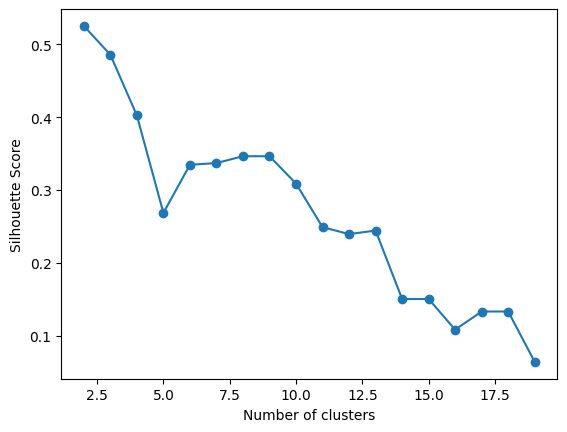
\includegraphics[width=\textwidth]{imgs/silhouette.png}
        \caption{Silhouette score across different k values.}
        \label{fig:silhouette}
    \end{minipage}
    \hfill
    \begin{minipage}[t]{0.48\textwidth}
        \centering
        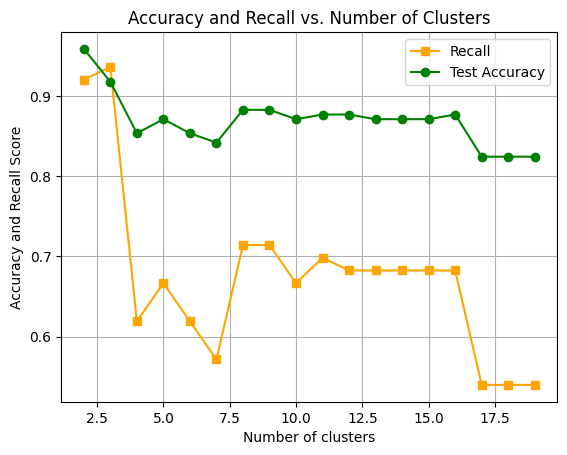
\includegraphics[width=\textwidth]{imgs/recall_test_acc.png}
        \caption{Recall and test accuracy score across different k values.}
        \label{fig:recall_test_acc}
    \end{minipage}
\end{figure}

\section{RBF Network Training}
\label{sec:rbf-network}
We built a custom RBF Network passing the \textbf{centre} and \textbf{sigma} parameters manually. The centres were the centroids from clustering when \textbf{k = 2}, which had the highest silhouette score. Sigma was the \textbf{euclidean distance} between the 2 centroids times the square root of 2. The last layer is 1 neuron with no activation function. As for the updating of the weights, \textbf{SSE} was the loss function and \textbf{Moore-Penrose pseudoinverse} the update rule. These were the results:
\begin{itemize}
    \item \textbf{Confusion matrix}: 
    \[
    \begin{array}{|c|c|c|}
    \hline
    & \textbf{Predicted Positive} & \textbf{Predicted Negative} \\
    \hline
    \textbf{Actual Positive} & 48 & 15 \\
    \hline
    \textbf{Actual Negative} & 2 & 106 \\
    \hline
    \end{array}
    \]
    \item \textbf{Accuracy}: 90.0\%
    \item \textbf{Recall}: 0.76\%
\end{itemize}

The performance in both accuracy and recall decreased when compared to the logistic regression in both the original and mapped datasets.  RBF Network uses the distance of the data points to the centres of the clusters. We can interpret each cluster centre as a feature. The closer a data point is to a cluster centre, the more it exhibits the characteristics of that feature. Since there are only two clusters, the model might be underfitting, as it relies on just two features (the centroids of the clusters).

To find out if having only 2 clusters creates difficulties in learning and causes underfitting, we decided to perform RBF Network across all k values. Then we plotted the results:
\begin{figure}[H]
    \centering
    \begin{minipage}[t]{0.48\textwidth}
        \centering
        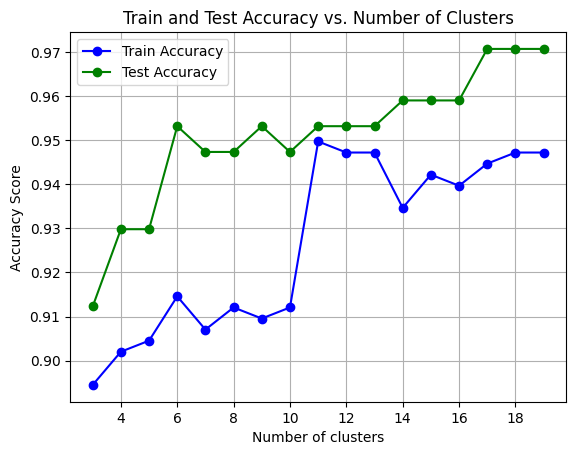
\includegraphics[width=\textwidth]{imgs/acc_rbf.png}
        \caption{Accuracy scores across different k values.}
        \label{fig:acc_recall}
    \end{minipage}
    \hfill
    \begin{minipage}[t]{0.48\textwidth}
        \centering
        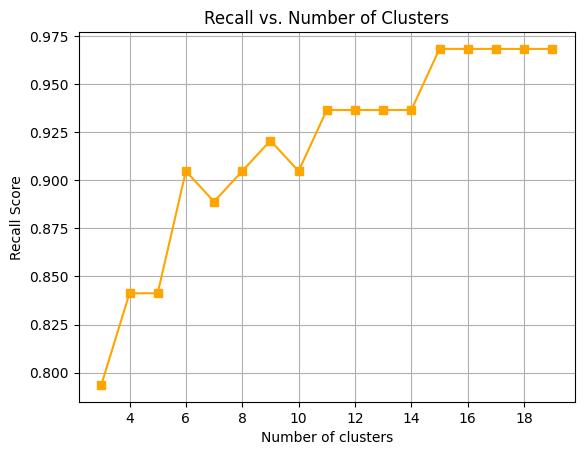
\includegraphics[width=\textwidth]{imgs/recall_rbf.png}
        \caption{Recall scores across different k values.}
        \label{fig:recall_rbf}
    \end{minipage}
\end{figure}


Despite some fluctuations, both accuracy and recall exhibit an overall tendency for improvement as the number of clusters increases (Fig. \ref{fig:acc_recall}). This trend suggests that a greater number of clusters enables the model to better capture the underlying complexity of the data, corroborating our hypothesis that using only two clusters on this model is insufficient for effectively learning the intricacies of the dataset.

Test accuracy was higher than train accuracy. This is an odd event since in our implementation of RBF Network we did not add any kind of regularization. Further more, after trying to spread and contract the sigma by multiplying and dividing by $\sqrt{2}$, respectively, the test accuracy remained higher than training accuracy. 

\section{Conclusion}
The model with the highest performance scores was logistic regression on the raw dataset and RBF Network with the highest k values (Figs \ref{fig:recall_test_acc} \& \ref{fig:acc_recall}). While these models had a very good performance, \textbf{they are hard to understand} as they have a high dimensionality. The logistic regression on the mapped dataset, specifically when \textbf{k = 2} and \textbf{k = 3}, had close results and the advantage of a \textbf{low dimensionality}, making it easy to understand its behaviour. This is a trade-off that must be weighed in when choosing a model. 
This situation reminds us that machine learning doesn't offer a one-size-fits-all solution, as different problems, conditions, and situations require varying priorities, making the right choices context-dependent.
\label{sec:conclusion}

\end{document}